\section{Detección de marcadores}
Una vez realizada la captura de video del paciente, el primer paso es reconocer los marcadores en el cuerpo del sujeto.

El bloque de detección de marcadores, se puede dividir en dos partes: la \textbf{segmentación} y el \textbf{filtrado de objetos}. En la Figura \ref{ejemploabelumbr2} se muestra el resultado del procesamiento de cada etapa.

El algoritmo realiza la detección siguiendo el siguiente proceso:

\begin{enumerate}
  \item Se recibe como entrada un video y este es separado en cada uno de sus cuadros.
  \item Se toma un cuadro y se lo segmenta utilizando umbralización de Otsu.
  \item A partir de la imagen segmentada, se identifican los marcadores.
  \item Se escribe la posición de los marcadores detectados para este cuadro en un archivo con formato XML.
  \item Se toma el siguiente cuadro y se repite el proceso a partir del paso 2.
\end{enumerate}

Este bloque fue implementado en lenguaje C++, debido a que es uno de los lenguajes de programación que cuenta con mayor cantidad de recursos para procesamiento de imágenes. En particular, se utilizaron las librerías \emph{OpenCV} \cite{opencv} y \emph{CVBlob} \cite{cvblob} ya que funcionan para las plataformas principales de PC y dispositivos móviles, y están diseñadas para tener una gran eficiencia computacional en las implementaciones.

\subsection{Descripción de las etapas de detección}
\subsubsection{Segmentación}
En lo que respecta al bloque de segmentación, se eligió utilizar la umbralización generando umbrales con el método de Otsu\cite{otsu} de tres clases.

Trabajar con tres clases permite ser un poco más flexible con los contrastes entre los marcadores y el resto de la imagen por lo que no sería estrictamente necesario, por ejemplo, que el traje del paciente y el fondo sean del mismo color.

\subsubsection{Filtrado}
La etapa de filtrado no es más que una clasificación de los objetos segmentados. Dado que los objetos a detectar tienen formas relativamente sencillas (círculos blancos sobre fondo oscuro) y las condiciones de laboratorio son controladas al realizar la captura, esta etapa no requirió implementar algoritmos muy complejos. En particular, se implementó un detector de objetos circulares en base a momentos geométricos\cite{imageMoments} y un filtro según el área de los mismos.

\subsection{Resultados}
Para la etapa de segmentación se observó que el resultado obtenido depende fuertemente de las condiciones de captura y del umbral calculado. Se debe tener especial atención en las condiciones de captura ya que de no cumplir con las establecidas los resultados no son del todo satisfactorios (ver Figura \ref{ejemploabelumbr2}). Por otro lado, si las capturas se hacen dentro de las condiciones establecidas, los resultados obtenidos son aceptables.

\begin{figure}[ht!]
      \centering
        \subfloat[]{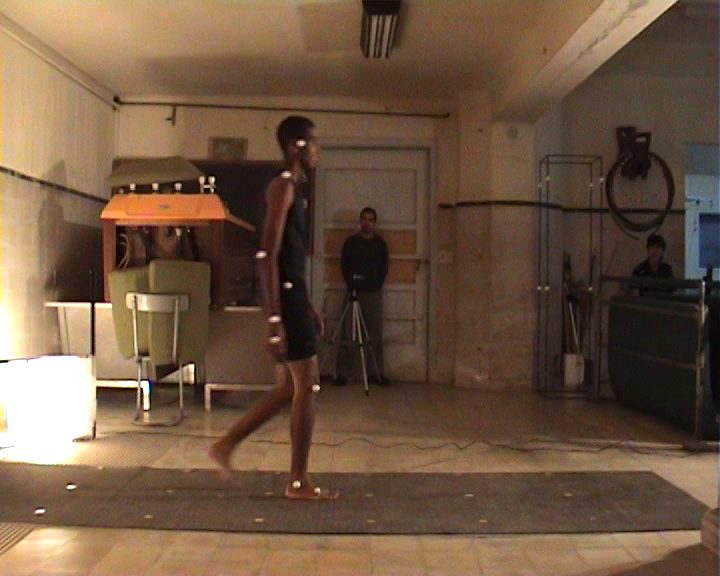
\includegraphics[scale=0.10]{imagenes/abel_original_video.png}\label{abelvideo}}\hspace{1 mm}
        \subfloat[]{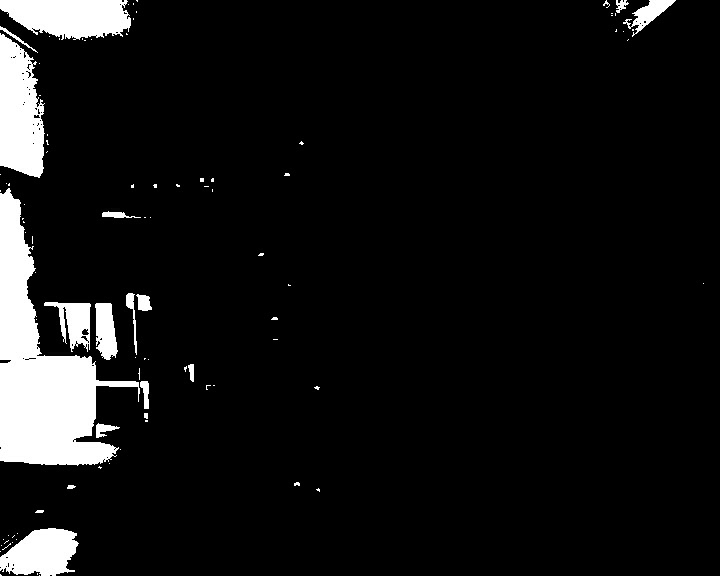
\includegraphics[scale=0.10]{imagenes/abel_original_filtro.png}\label{abelfiltro}}

        \subfloat[]{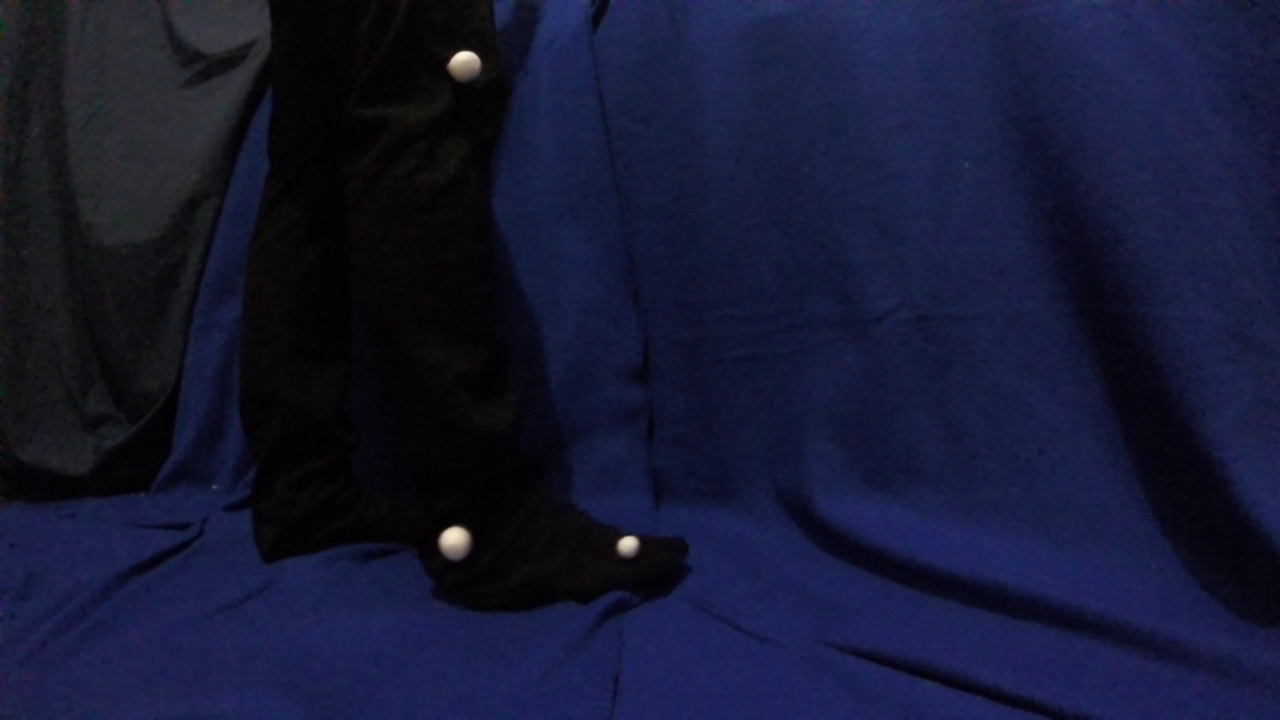
\includegraphics[scale=0.07]{imagenes/orig.png}\label{abelvideo2}}\hspace{1 mm}
        \subfloat[]{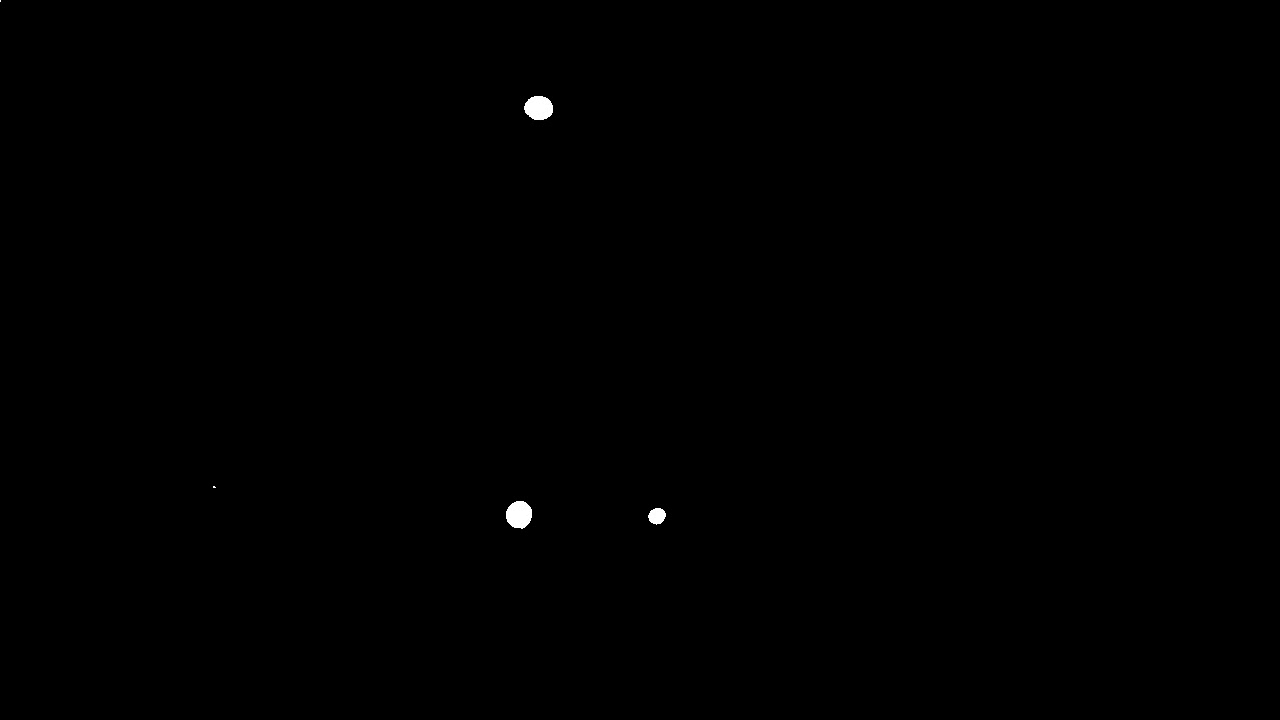
\includegraphics[scale=0.07]{imagenes/filtr.png}\label{abelfiltro2}}\hspace{1 mm}
        \subfloat[]{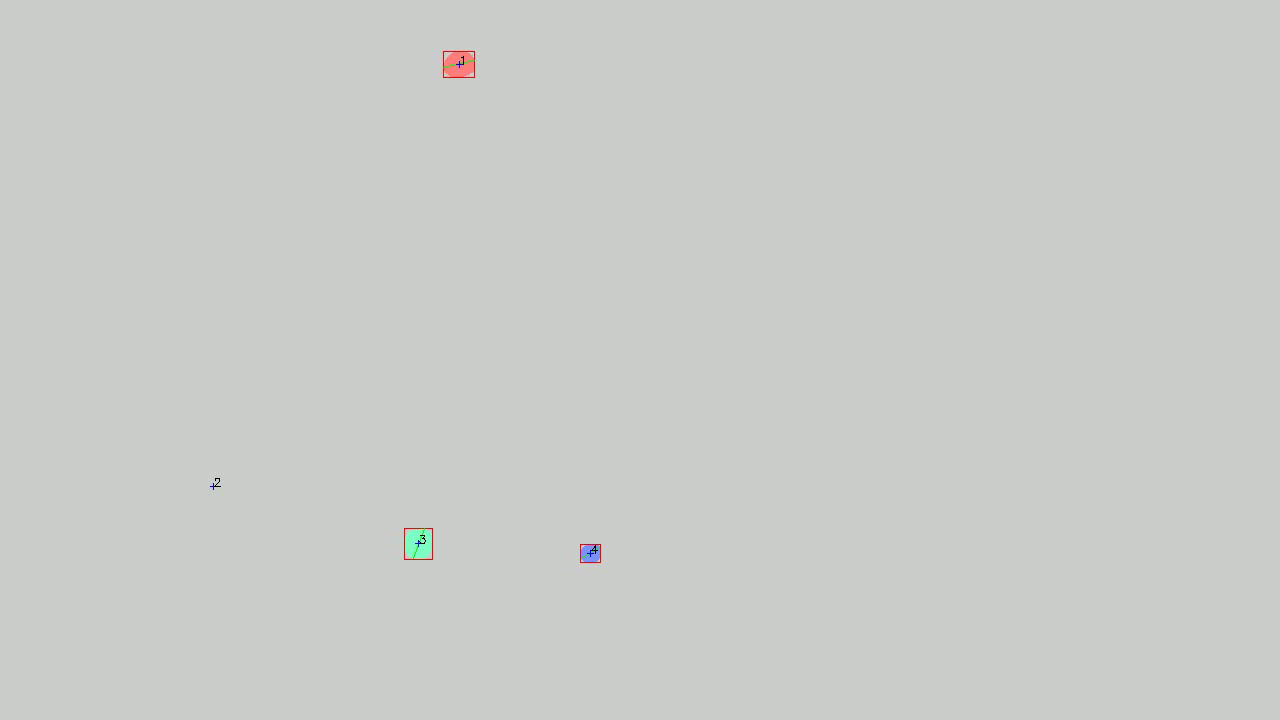
\includegraphics[scale=0.07]{imagenes/detect.png}\label{abeldetect}}
      \caption{Entradas y salidas de cada etapa del bloque de deteción. \textbf{(\ref{abelvideo})} Imagen original de una secuencia fuera de las hipótesis de captura. \textbf{(\ref{abelfiltro})} Imagen segmentada con el umbral de Otsu. \textbf{(\ref{abelvideo2})} Captura original de una secuencia real bajo las hipótesis de captura. \textbf{(\ref{abelfiltro2})} Imagen filtrada con el umbral de Otsu. \textbf{(\ref{abeldetect})} Marcadores detectados.}  
      \label{ejemploabelumbr2}
\end{figure}
